\subsection{Ejercicio 7}
\graphicspath{ {img/07} }

Thunderbird es un lector de correo con un gran número de funcionalidades adicionales, como calendarios, contactos y, más importante en nuestro caso, permite utilizar PGP para cifrar y firmar los correos.

Para añadir las claves se utiliza la herramienta \texttt{Gestor de claves PGP}, donde se pueden importar tanto los pares de claves completos como solo las claves públicas, como se muestra a continuación:

\begin{figure}[H]
    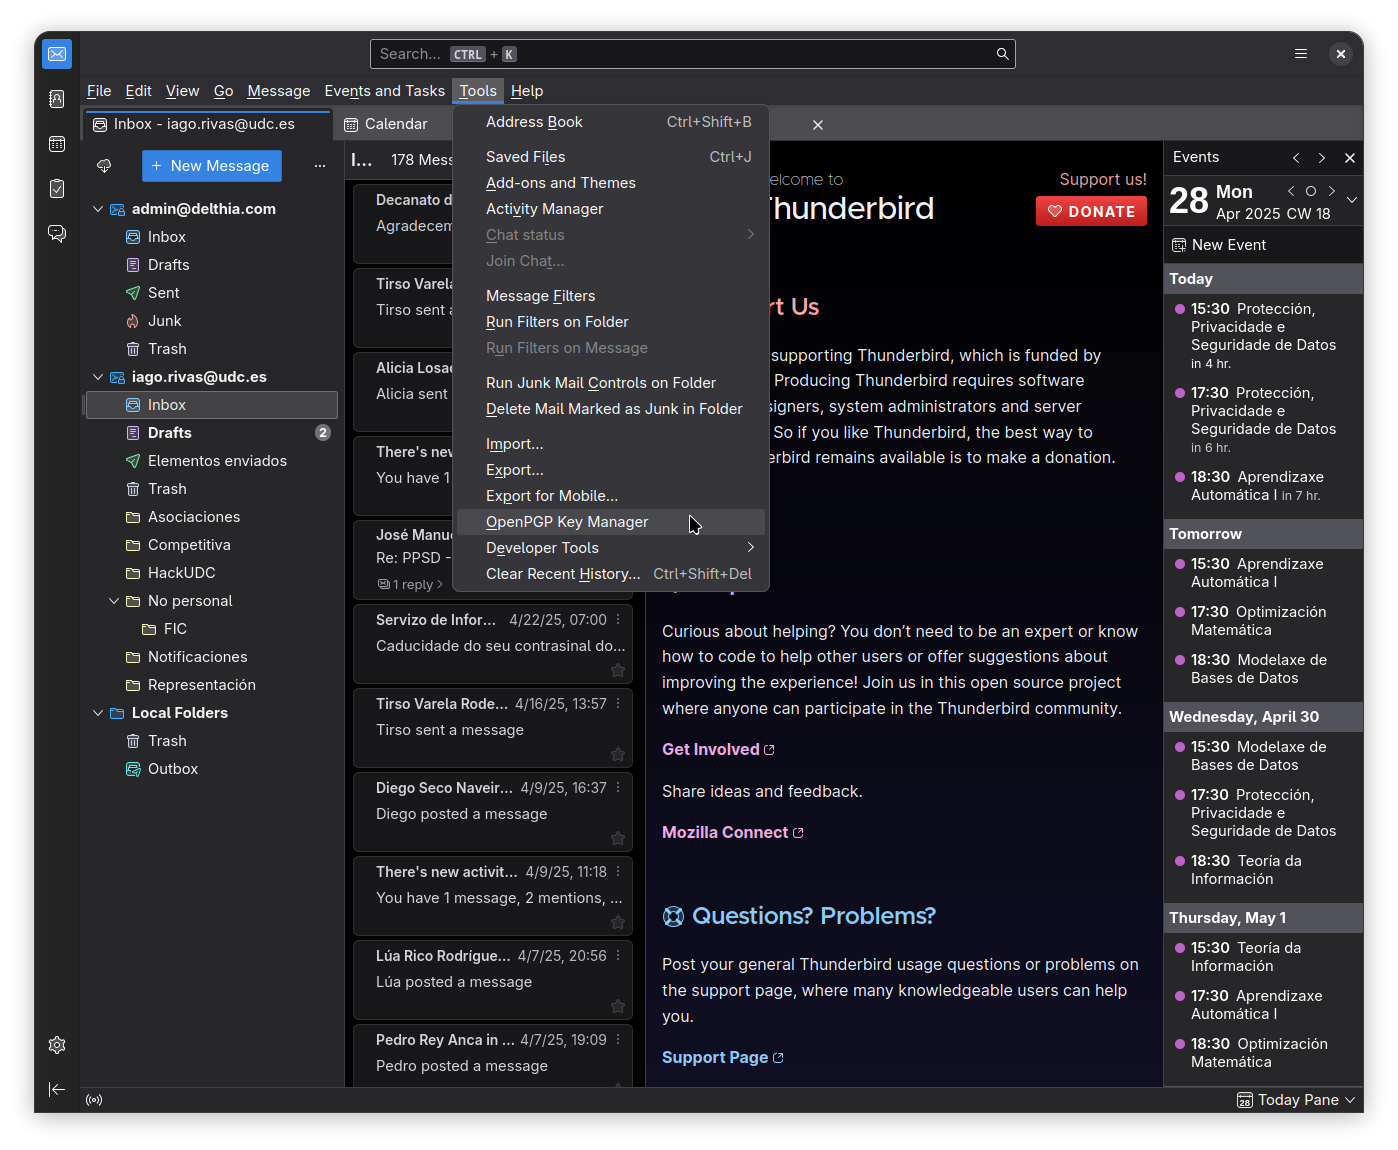
\includegraphics[width=15cm]{thunderbird-tools-menu.png}
    \caption{Menú con la herramienta "Gestión de claves OpenPGP"}
\end{figure}

\begin{figure}[H]
    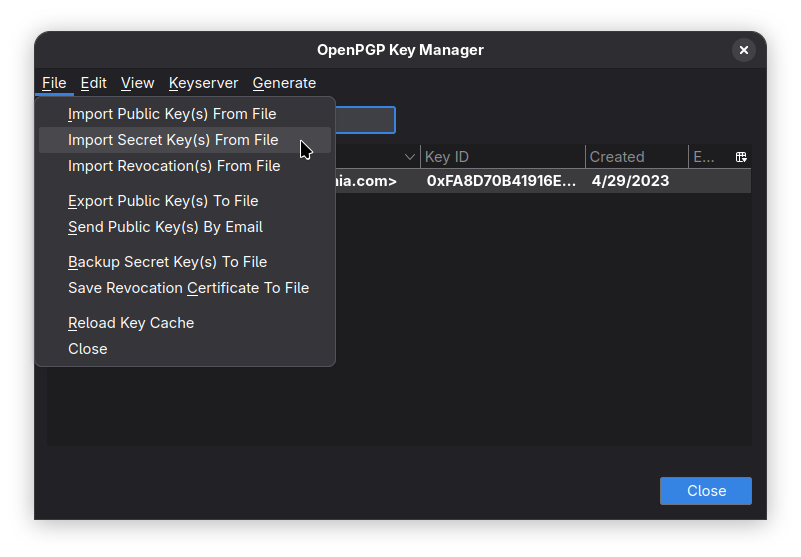
\includegraphics[width=15cm]{thunderbird-keymanager.png}
    \caption{Importación de claves en la herramienta "Gestión de claves OpenPGP"}
\end{figure}

Ahora, encriptar un correo es cuestión de selecciónar la opción "Encriptar" que se habilitará en la ventana de redacción, justo al lado del botón enviar. Junto a este botón hay un desplegable con tres opciones:
\begin{itemize}
    \item{\underline{Firmar:} Firma el correo con la clave del remitente. No afecta a la capacidad de leer el correo del destinatario.}
    \item{\underline{Encriptar:} Encripta el correo con la clave del destinatario, por lo que es necesario conoecer la clave pública del mismo. Además, el destinatario no podrá leer el correo sin desencriptarlo con su clave privada. Existe una opción que permite encriptar también el asunto}
    \item{Firmar y encriptar: Primero se firma el correo y luego se encripta. Esto permite mantener la privacidad en la comunicación y que solo el destinatario, que puede leer el correo, pueda comprobar también que el remitente es quien dice ser}
\end{itemize}

En estos casos el mensaje se envía como un bloque cifrado, y en caso de solo firmarse, se adjunta la firma. En otro lector de correo, por ejemplo la versión web de outlook, no podremos leer el mensaje y tendremos que descargarlo para desencriptarlo con \texttt{gpg}, mientras que Thunderbird muestra automáticamente los mensajes cifrados como si no lo estuvieran, además de indicar claramente si tienen una firma y si es válida.